\chapter{Nanowire Structure and Measurement}
In this chapter, we present the experiment data and some analysis which are the foundation of our circuit design.
The first section gives a brief description of our silicon nanowire element.
The second section provides the data of the biology experiments.
The last section presents the data of the electrical measurement, on which our circuit design spec depends.

\section{Brief Description of Nanowire Structure}
The nanowire we use is made by Prof.Yang's team (National Chiao Tong University)\cite{C5}.
Fig.\ref{fig:drawing} is the sectional view of the nanowire structure.
The fabrication process is based on the poly silicon sidewall spacer technique.
The n-Type doped poly-SiNW FET has two to ten poly silicon channels.
Each channel is 80nm in width and 2µm in length.
A Large portion of the channel surface is exposed to environment.
The exposed region, through several post-process, capture the DNA probe and serve as the sensing site for DNA molecules.\cite{C5, C6}


\begin{figure}[!htbp]
    \centering
    \begin{minipage}[t]{0.4\textwidth}
        \includegraphics[width=1\linewidth]{images/chapter3/Nw.png}
        \raggedleft
        (a)
    \end{minipage}
    \vfill
    \vfill
    \begin{minipage}[t]{0.4\textwidth}
        \includegraphics[width=1\linewidth]{images/chapter3/Nw_section.png}
        \raggedleft
        (b)
    \end{minipage}
    \caption{Nanowire Structure.  (a) A nanowire element with two poly silicon channels. (b) is the sectional view of the cutting plane in (a). }
    \label{fig:drawing}
\end{figure}


\section{Biology Experiment}
The biology experiment data are provided by Prof.Yang's team.
These data are the Id-Vg measurement of the same biomolecule placed under different circumstances or with different nanowire elements.
With each measurement repeated three times, we find the mean and standard deviation (SD) of them and consider the SD value as the intrinsic noise of nanowire.
We want to ensure that such noise should not be greater than the signal.
To be more specific, we examine whether the Id-Vg curves of different concentration overlap with each other or not.
We present an example below:
%ghas
\begin{figure}[!htbp]
    \centering
    \begin{minipage}[t]{0.4\textwidth}
        \centering
        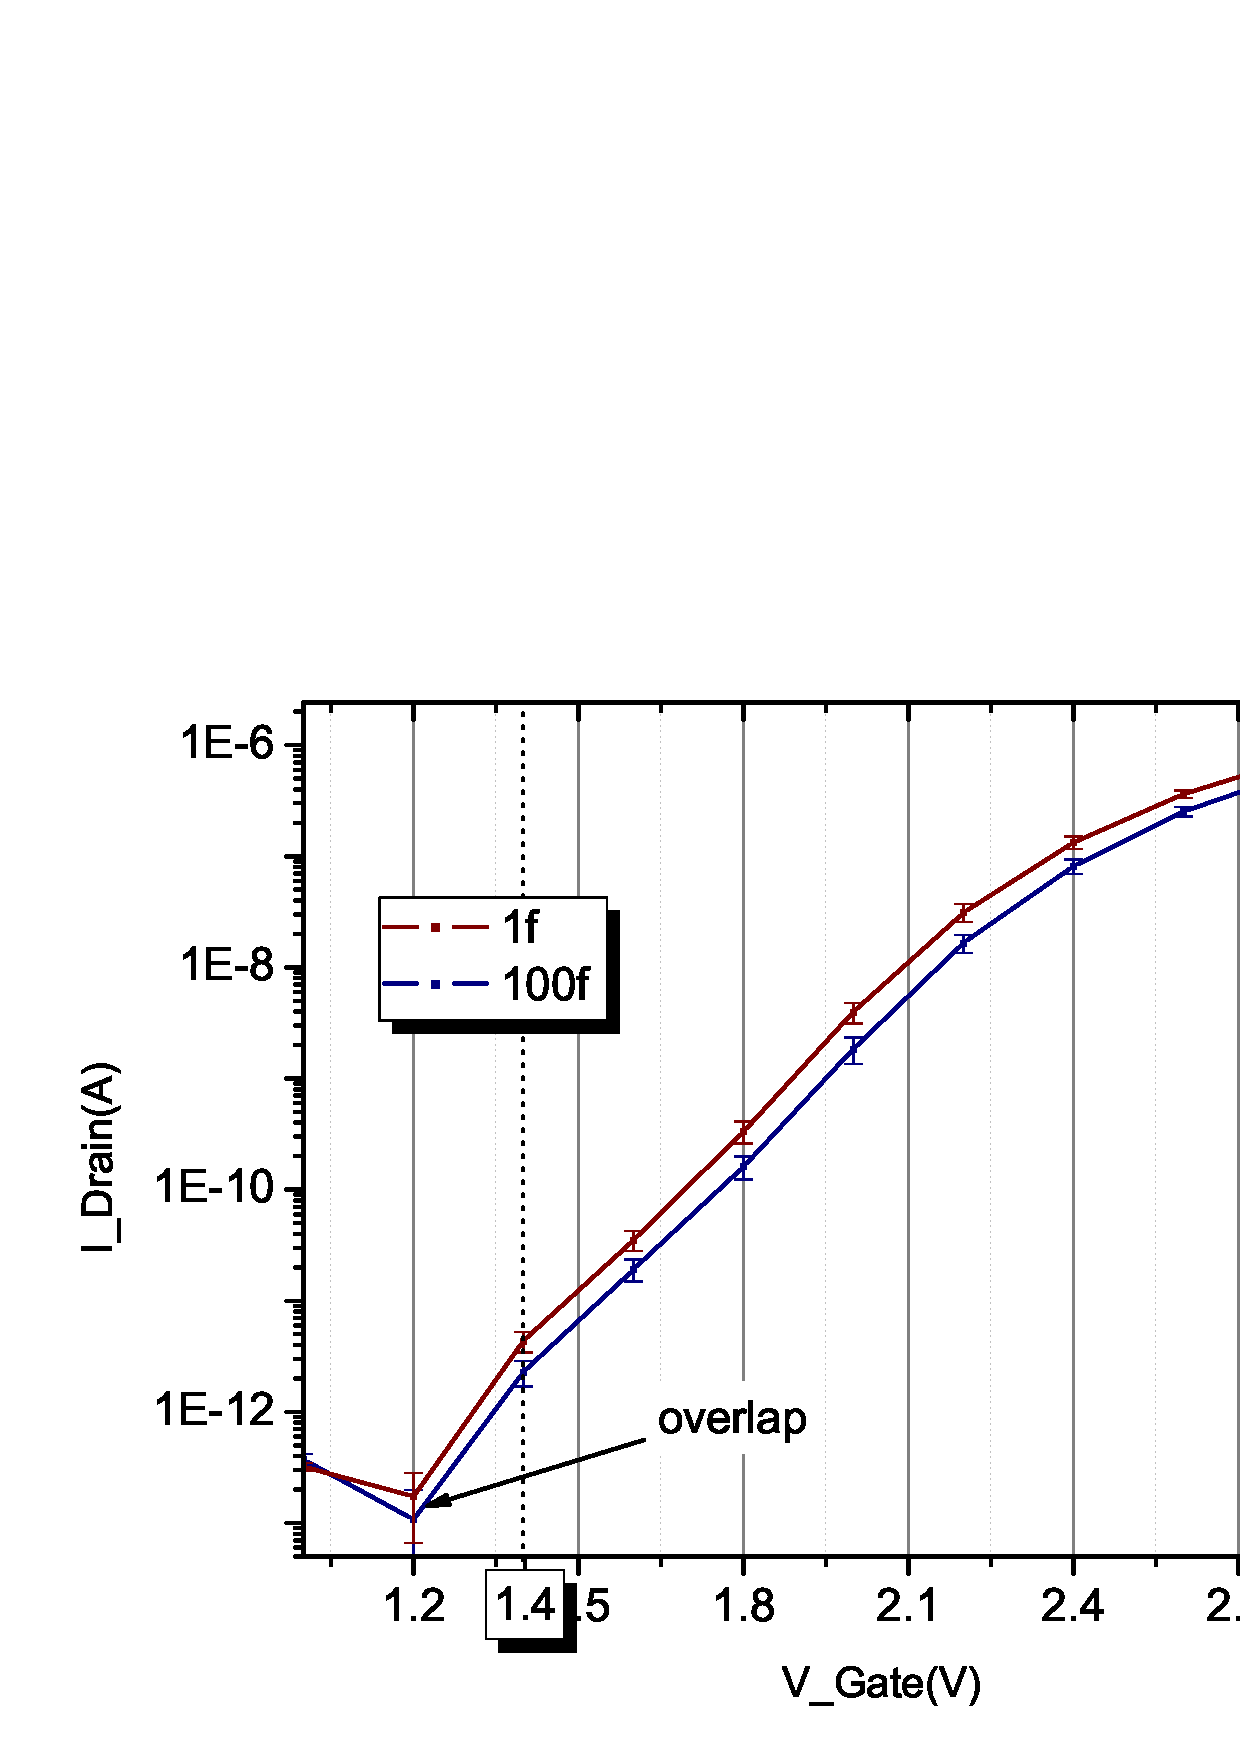
\includegraphics[scale=0.3]{images/chapter3/208_devices/L2-8_log.png}
        (a)
    \end{minipage}
    \hfill
    \begin{minipage}[t]{0.4\textwidth}
        \centering
        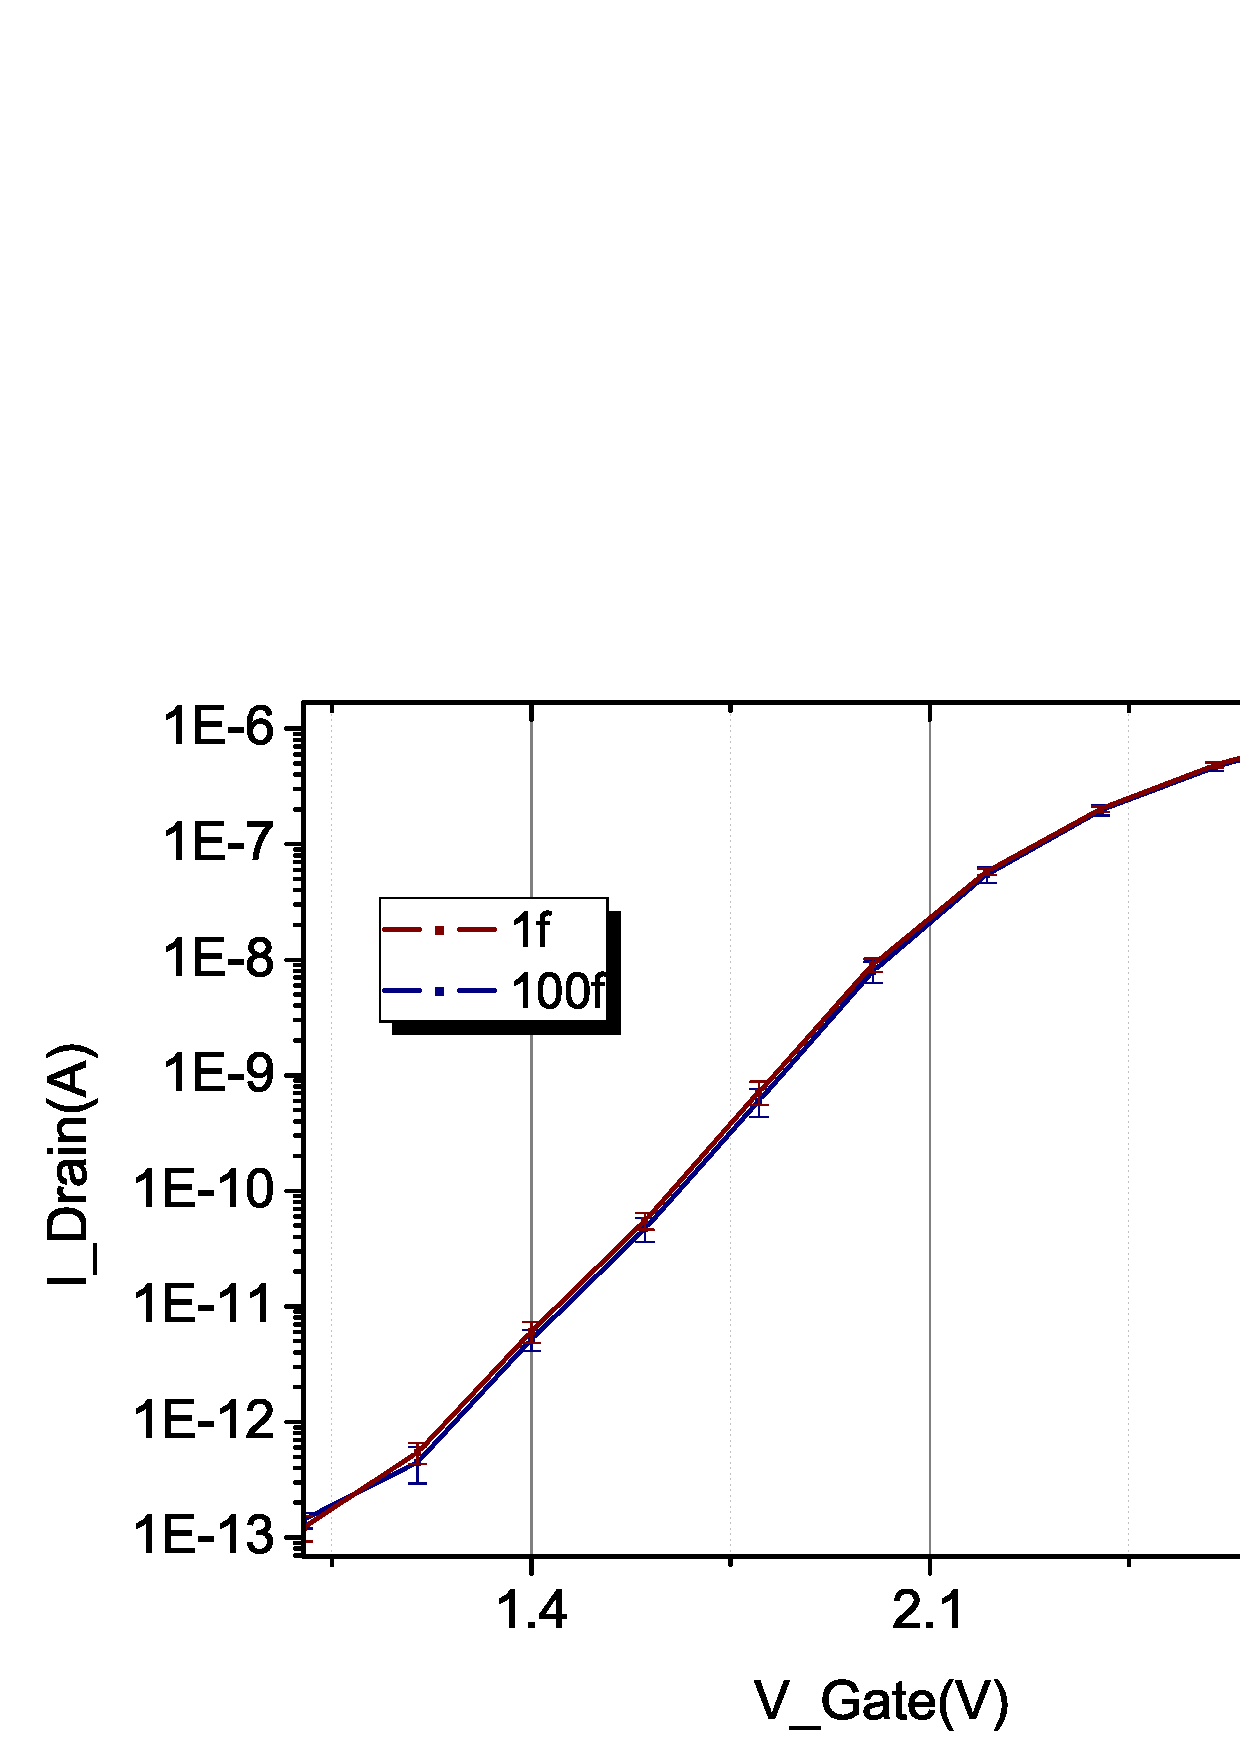
\includegraphics[scale=0.3]{images/chapter3/208_devices/L2-10_log.png}
        (b)
    \end{minipage}
    \caption{Concentration-dependent $I_D$-$V_G$ curves of two equivalent nanowire elements.
    In (a), the measurement result of 1fM and 100fM biomolecule solution is distinguishable. There is no overlap between two curves. This is not true in (b).}
    \label{fig:SD_sucandfail}
\end{figure}

Fig.\ref{fig:SD_sucandfail} are concentration-dependent measurements (1 femto mole(fM) and 100fM biomolecule solution) obtained with two elements ((a) and (b)).
The two curves in the (a) are distinguishable from the other after gate voltage of 1.4v
They are not distinguishable in the (b) since they overlap each other.
We thus assert that the element of (b) can't detect the concentration difference between 1fM and 100fM.
The noise is stronger than the signal (The signal means the $I_D$ difference caused by the concentration difference).
The element of (a) can do so if it is biased at gate voltage larger than 1.4v or drain current larger than 1E-11.

\begin{figure}[!htb]
        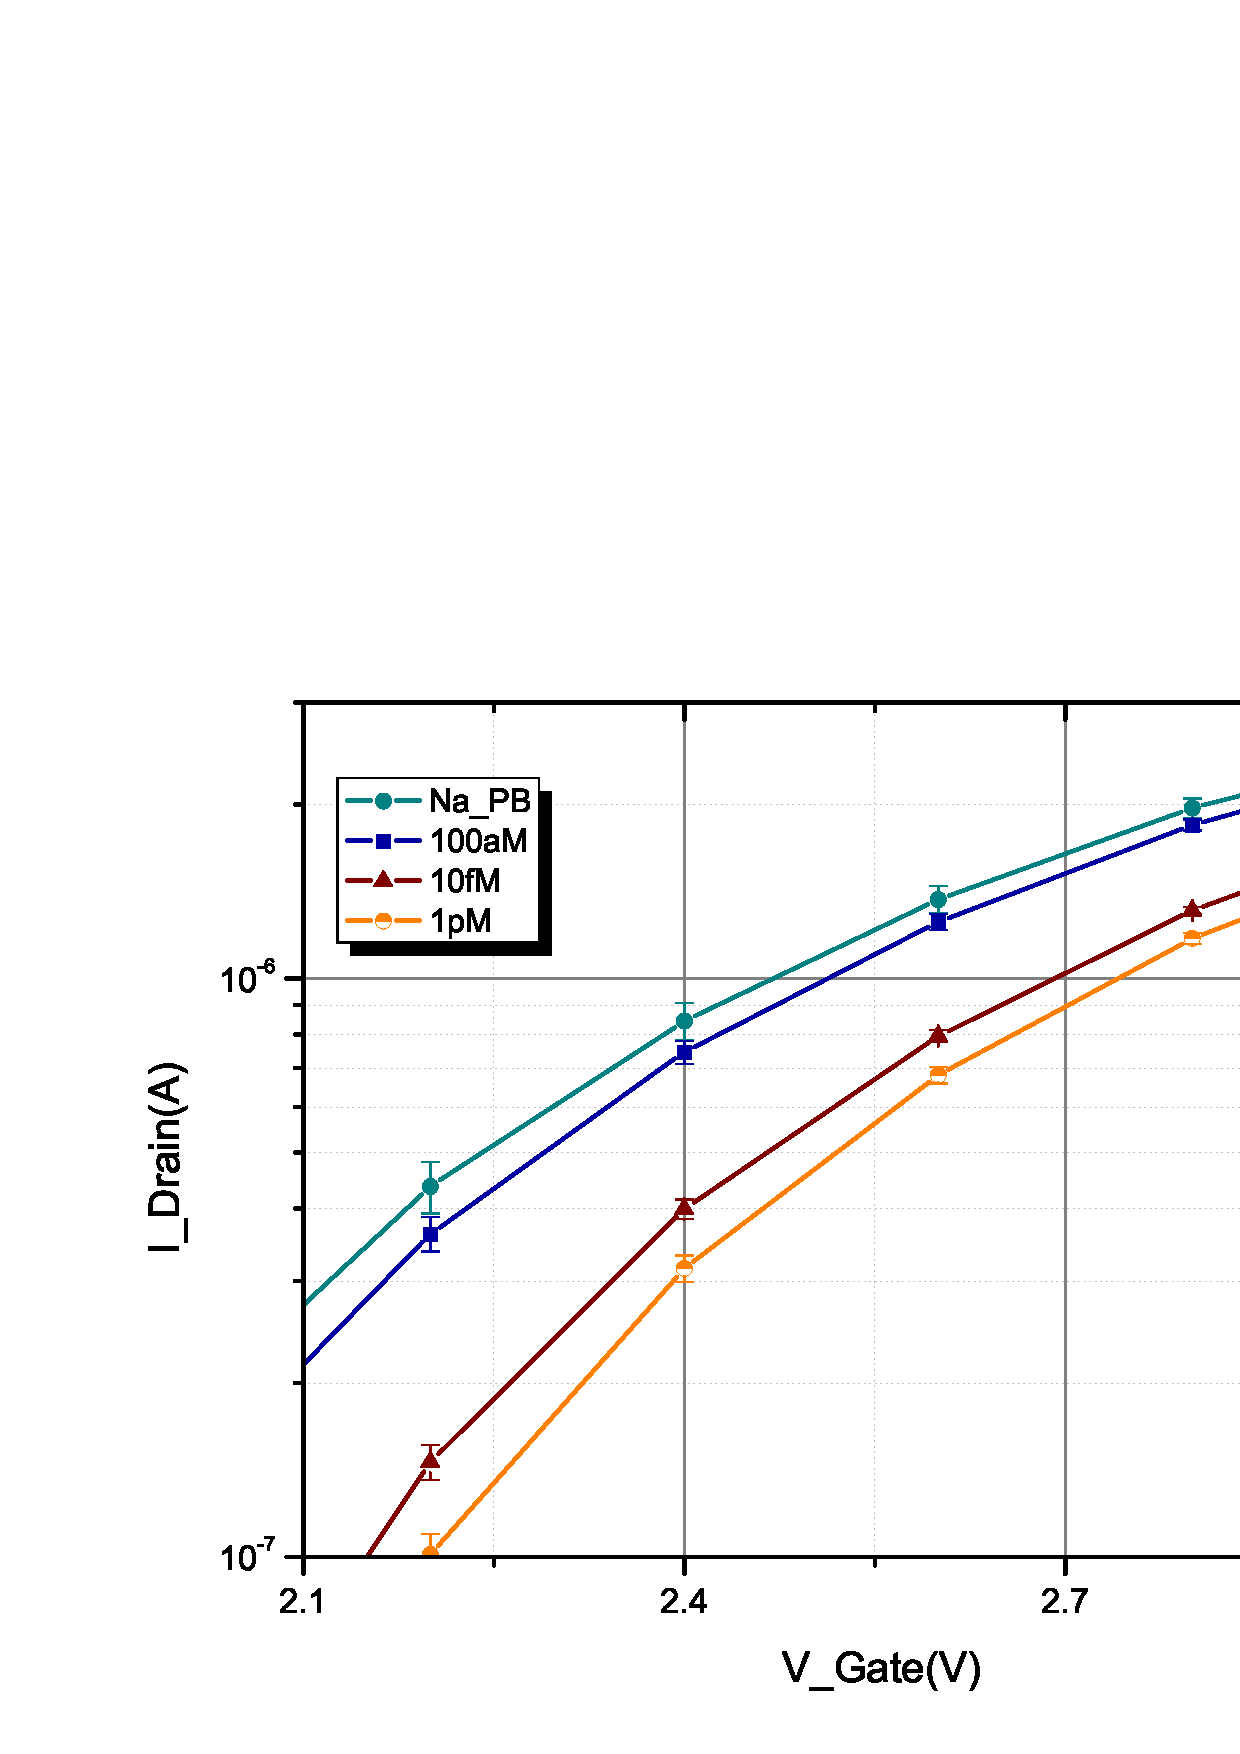
\includegraphics[width=1\textwidth]{images/chapter3/128_allT_mag.png}
    \caption{Concentration-dependent $I_D$-$V_G$ curves with concentration of Na\_PB(Buffer solution only), 100aM, 10pM, 1pM.
    Since the biomolecule is negative-charged, the lower the concentration is, the higher the curve is.
    To be noticed, the 10fM curve is closer to the curve of 1pM than 100aM.
     }
    \label{fig:SD_allT}
\end{figure}

In Fig.\ref{fig:SD_allT}, $I_D$ increase with the biomolecule concentration.
One can find that there is only a few ``space'' between PBS buffer and solution containing biomolecule with the concentration of 100aM.
Hence the 100aM should be the limit of detection.

It is worth noting that there is more space between 100aM and 10fM than the space between 10fM and 1pM.
And the noise rate: ${SD} / {Mean}$ is independent of concentration (Fig.\ref{fig:SD_allT2}).
Hence we say that the ``resolution'' for detecting concentration ranging from 100aM to 10fM may be better than the that ranging from 10fM to 1pM.
\begin{figure}[!htbp]
        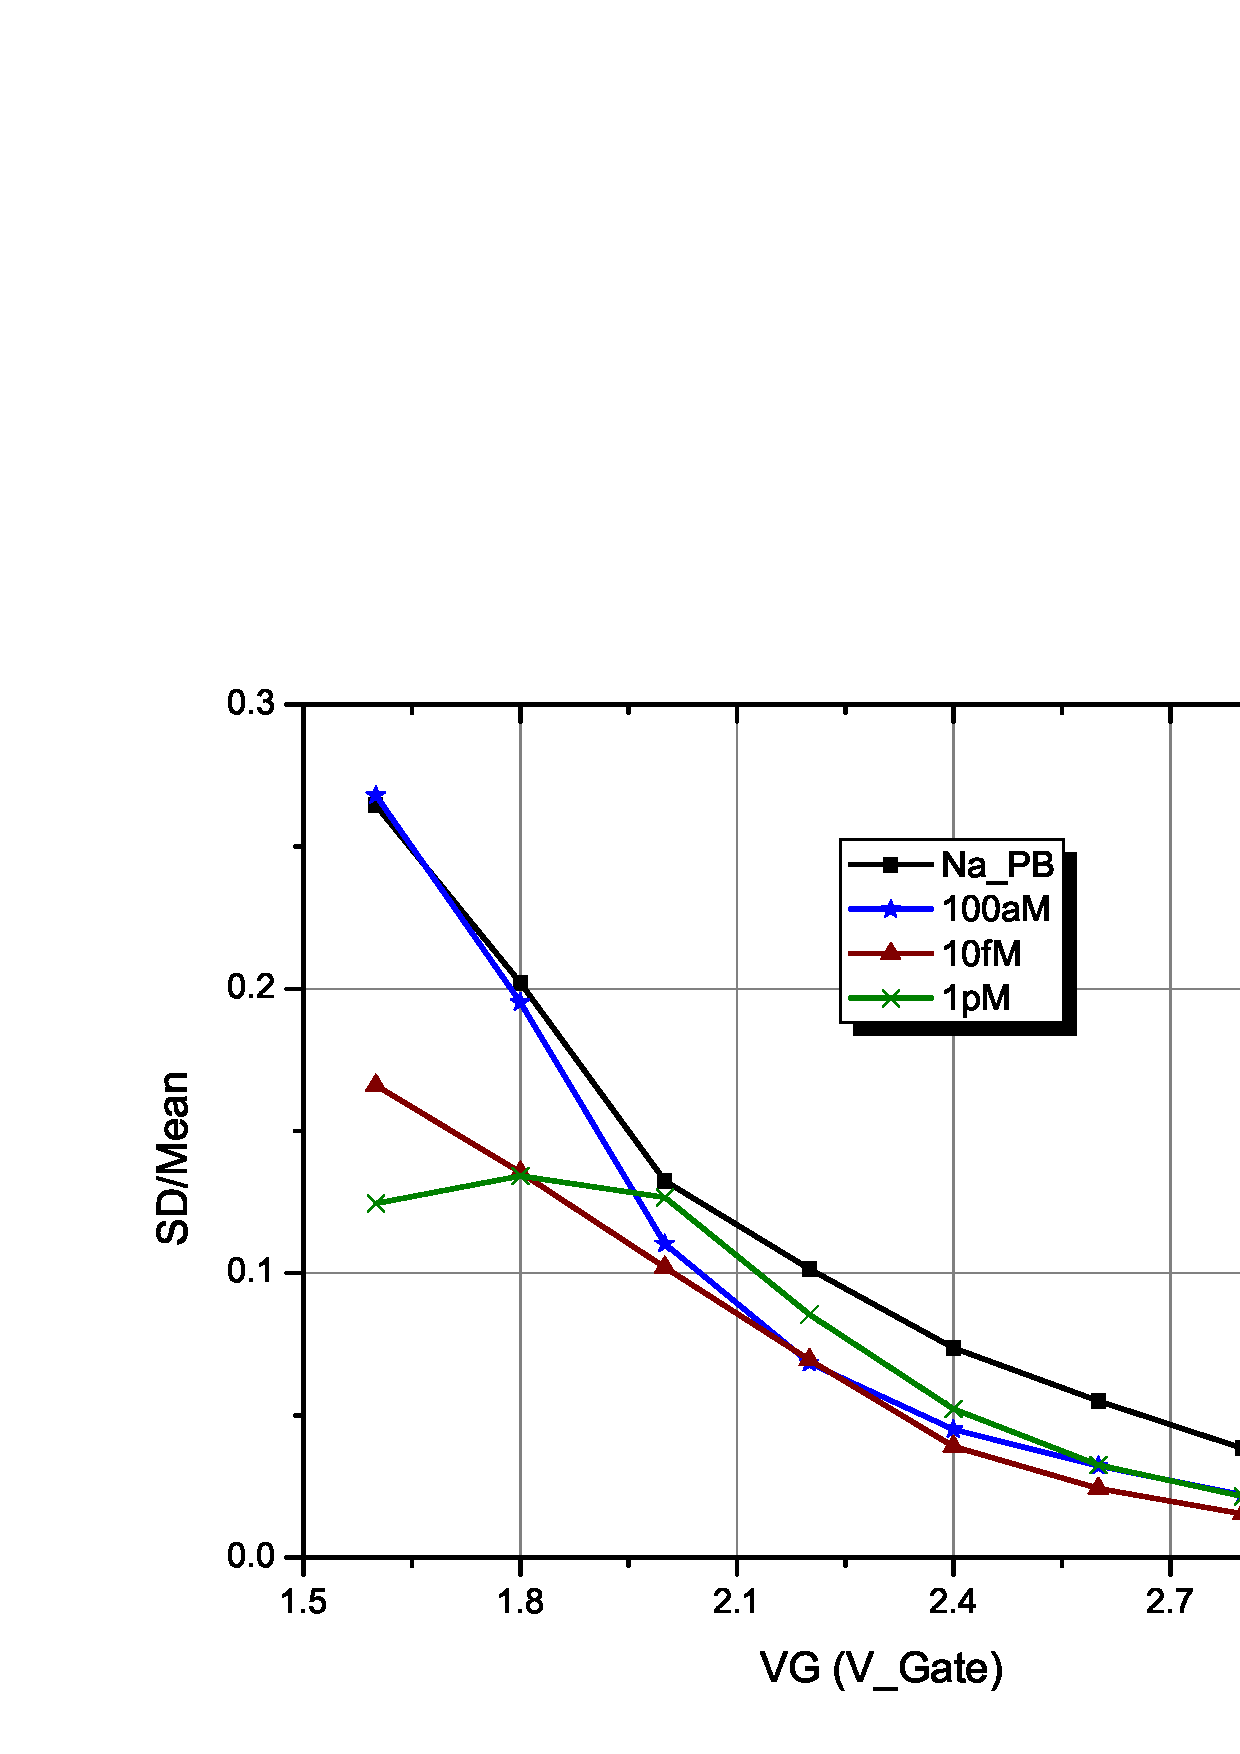
\includegraphics[width=1\textwidth]{images/chapter3/128_allT_error.png}
    \caption{The noise rate of Fig.\ref{fig:SD_allT}. The noise rate is obtained by dividing SD by Mean.}
    \label{fig:SD_allT2}
\end{figure}

\subsection{Appropriate operation region} \label{section:biasVg}
In \cite{C6}, the team found that ``the induced change of current ($I_D$) following biomolecule was dependent on the applied gate voltage (VG)'' (Fig.).
In other words, a ``biomolecule concentration resolution'' seems to depend on $V_G$
The team tried to find a bias gate voltage range which can induce more current response.
In our opinion, the induced change of current ($I_D$) following biomolecule is not directly dependent on $V_G$.
Based on the our assumption 2 (section\ref{section:twqAssumption}), it depends on the transconductance.
The phenomenon is found by $I_D$-$V_G$ curves, which means the $V_G$ also affect the $I_D$ which cause different transconductance.

Furthermore, we think the noise effect should be taken into consideration.
Some kinds of noise have  positive correlations with transconductance.

Still, we want to find an appropriate operation region of nanowire that has the largest concentration resolution.
We proposed a comprehensive method that one should choose the operation region with more ``noise tolerance''.
The noise tolerance is defined as:
\setlength{\mathindent}{2cm}
\begin{align}
    noise \quad tolerance = \frac{I_D1 - SD1 - (I_D2 + SD2)}{I_D2}
\end{align}
$I_D$ and $SD$ are the mean and standard deviation of a curve.
The larger the noise tolerance implies there is more space between two curves.
And more space implies the less chance of overlapping between to concentration curves may happens.

We present analysis results from three nanowire elements.
Fig.\ref{fig:SD_Device}(a), (c), (e) are the $I_D$-$V_G$ curves of three elements and Fig.\ref{fig:SD_Device}(b), (d), (f) are the noise tolerance respectively.
One can observe in (b) and (d) that there is first a rising trend then followed by a drop as gate voltage decreases.
The drop doesn't exist in (f) may because the weak inversion is too narrow.
The transistor enters into the reverse region before the drop appears.
The highest points of (b) and (d) locate in the weak inversion region and is close to the transition region (The region between strong inversion and weak inversion region).
We therefore suggest that in this section nanowire should has the largest concentration resolution.



\begin{figure}[h!]
    \centering
    \begin{minipage}[t][20cm][t]{1\textwidth}
        \begin{minipage}[t]{0.3\textwidth}
            \centering
            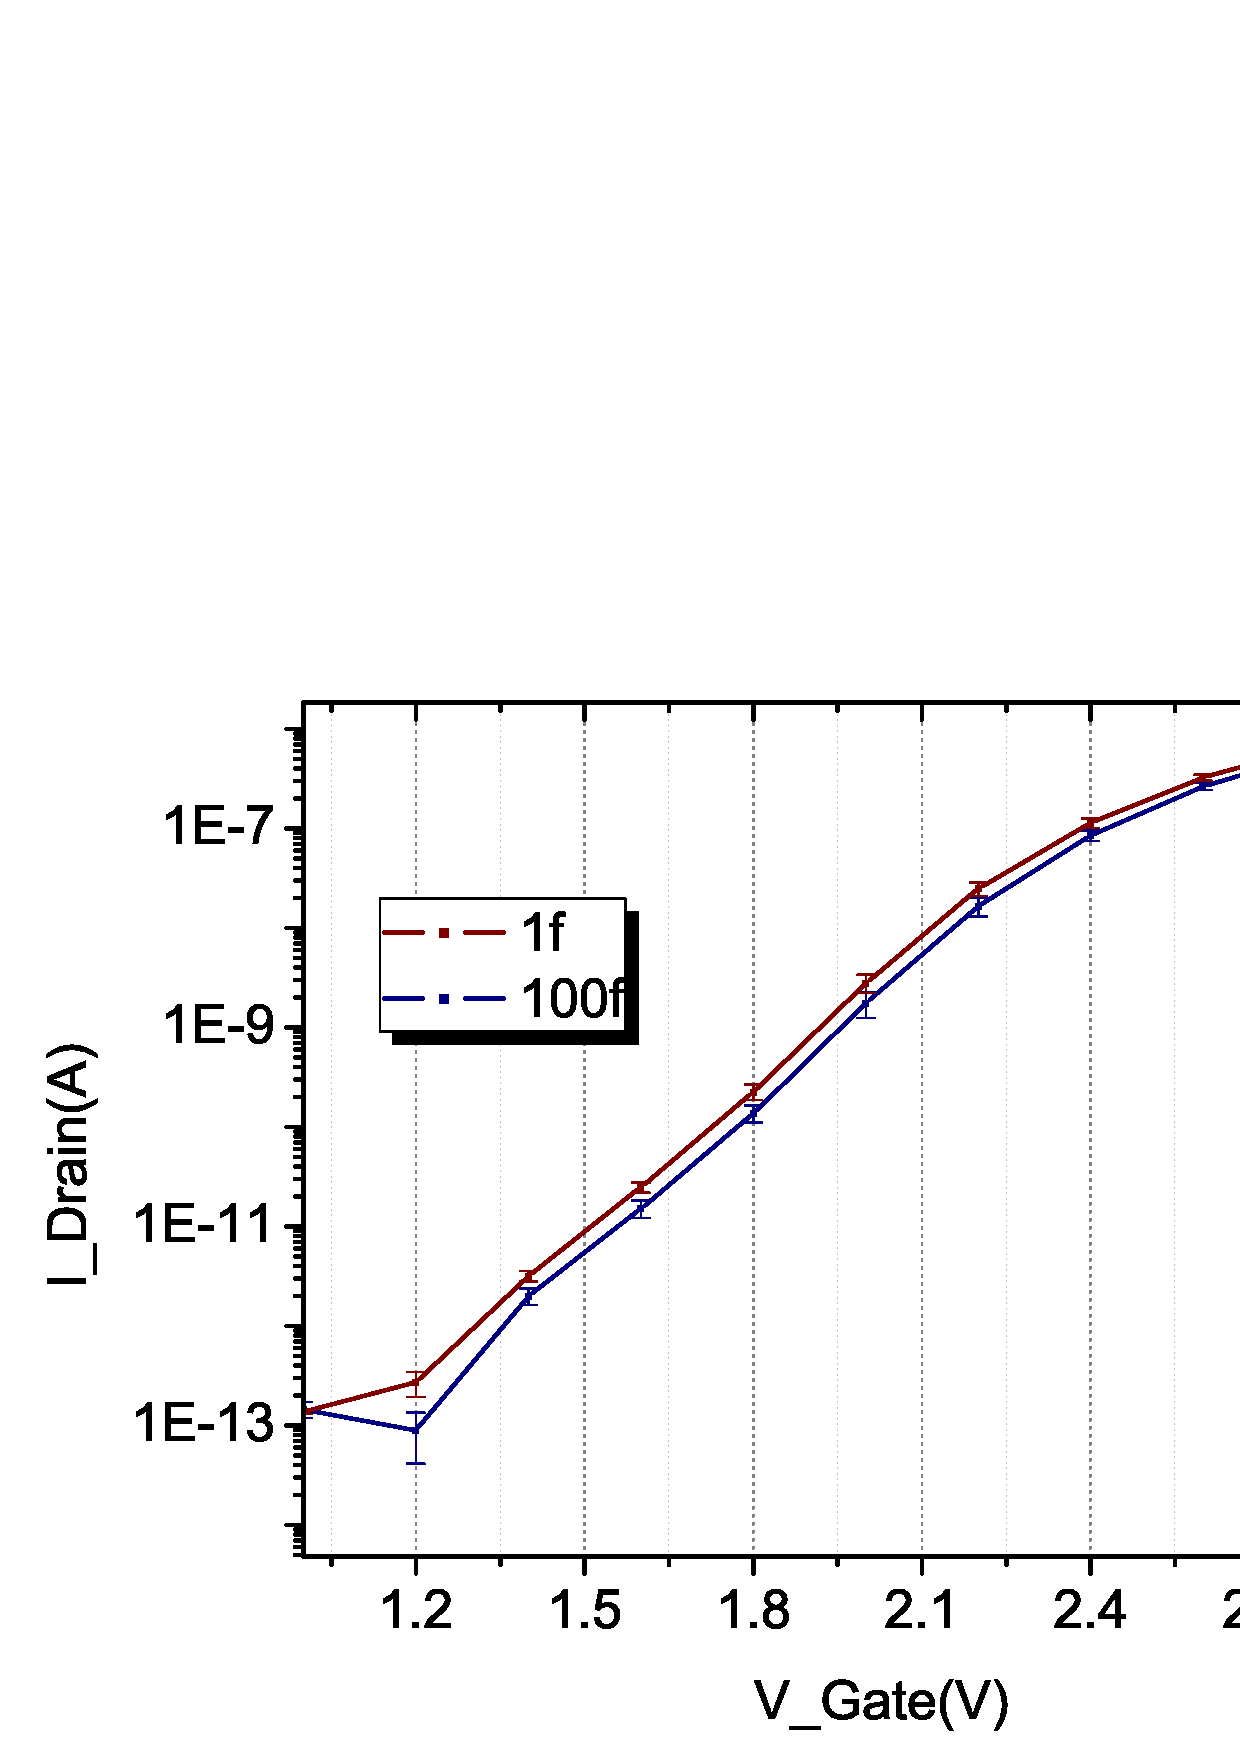
\includegraphics[width=1.8\textwidth]{images/chapter3/208_devices/L2-7_log.png}
            (a)
        \end{minipage}
        \hfill
        \begin{minipage}[t]{0.3\textwidth}
            \centering
            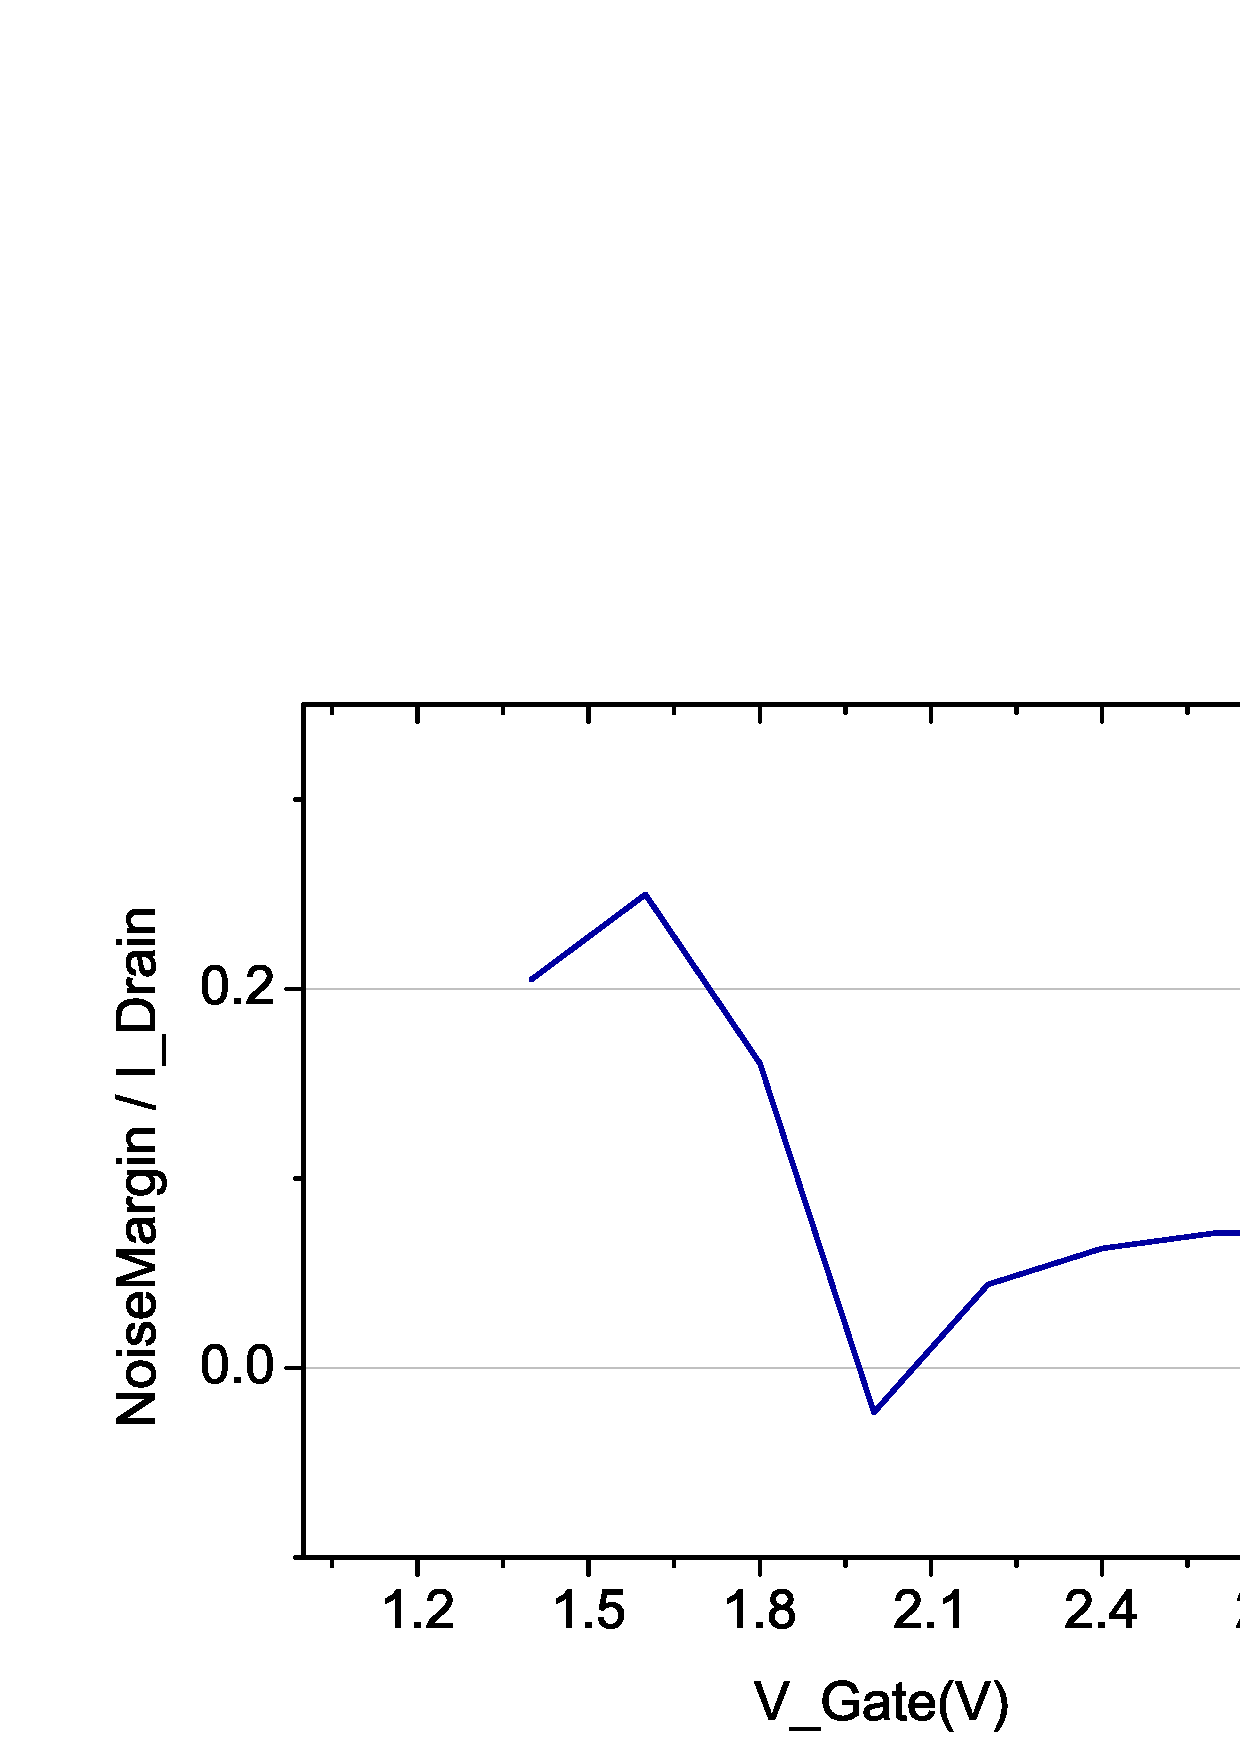
\includegraphics[width=1.6\textwidth]{images/chapter3/208_devices/L2-7_margin.png}
            (b)
        \end{minipage}
        \vfill
        \begin{minipage}[t]{0.3\textwidth}
            \centering
            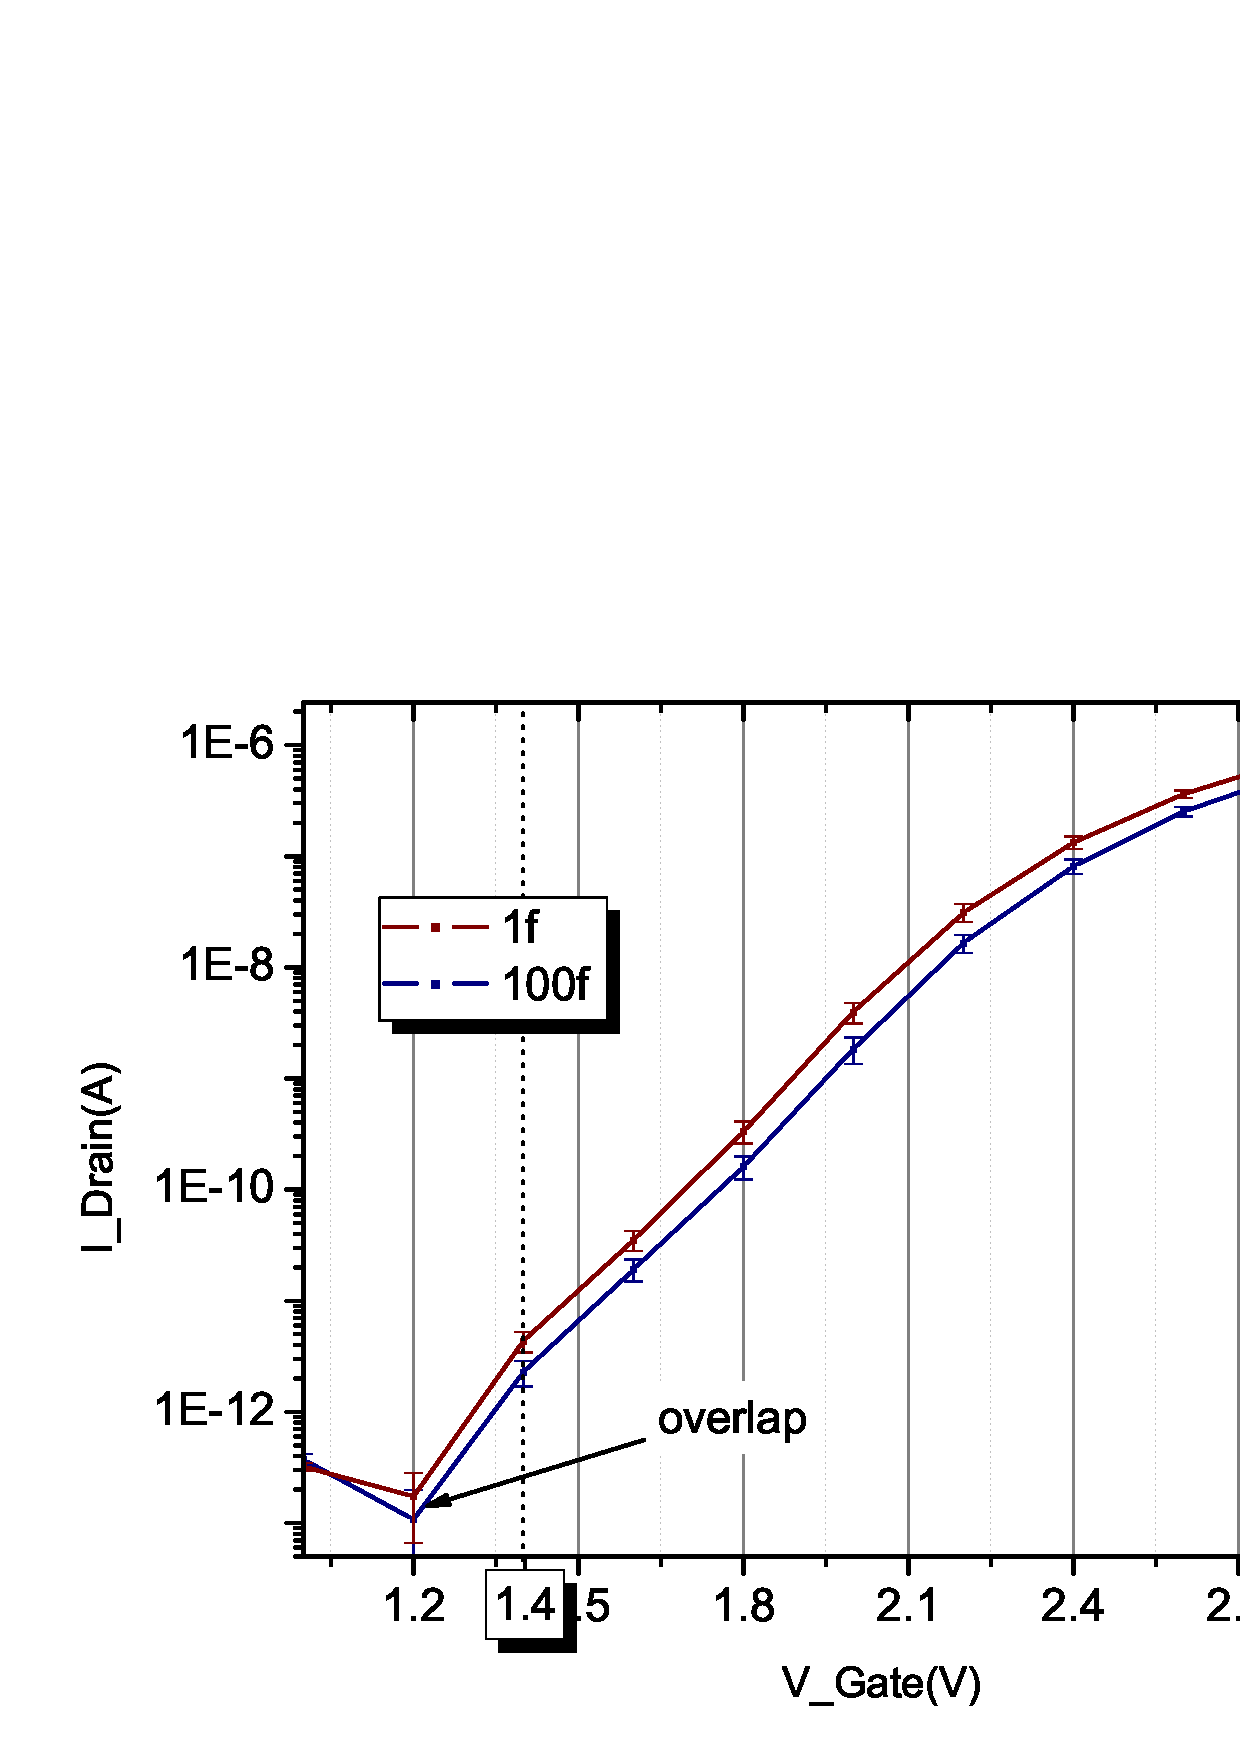
\includegraphics[width=1.8\textwidth]{images/chapter3/208_devices/L2-8_log.png}
            (c)
        \end{minipage}
        \hfill
        \begin{minipage}[t]{0.3\textwidth}
            \centering
            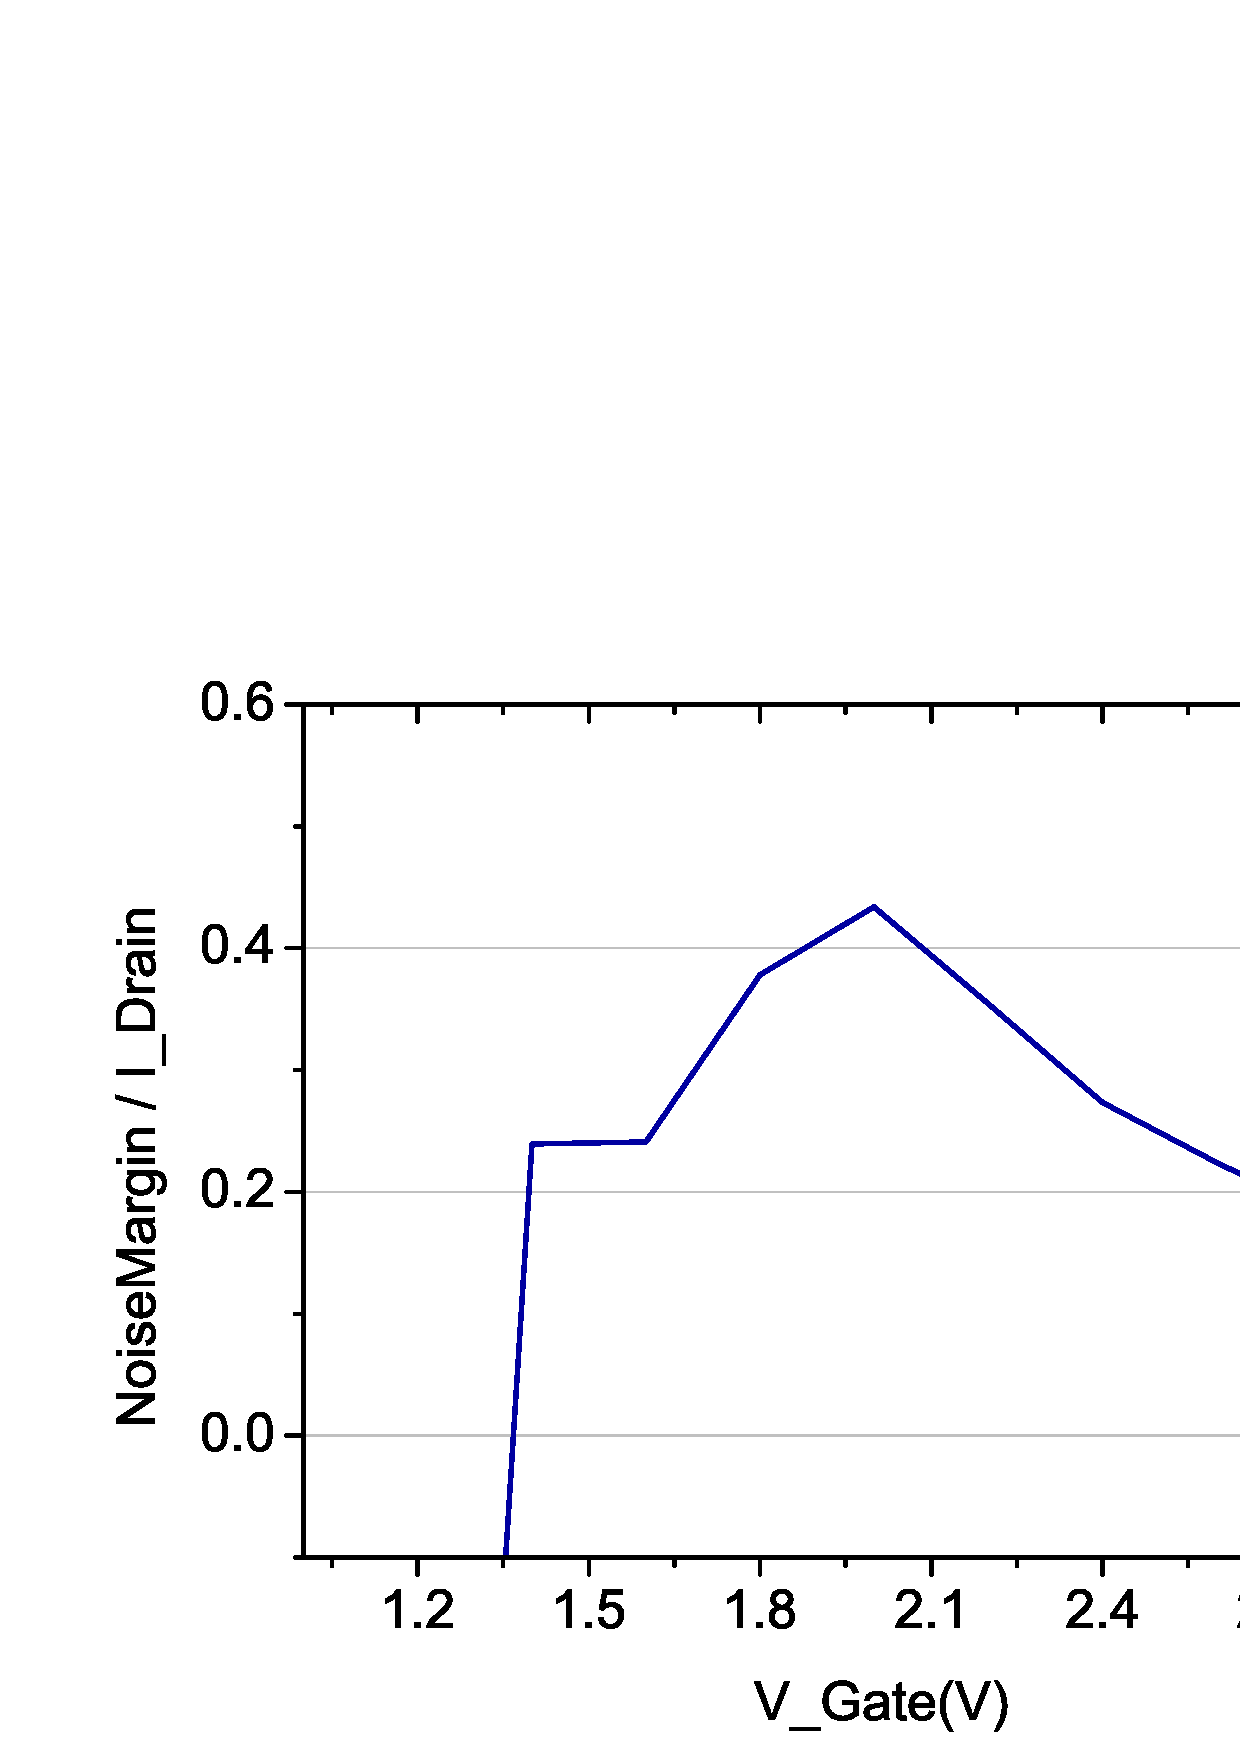
\includegraphics[width=1.6\textwidth]{images/chapter3/208_devices/L2-8_margin.png}
            (d)
        \end{minipage}
        \vfill
        \begin{minipage}[t]{0.3\textwidth}
            \centering
            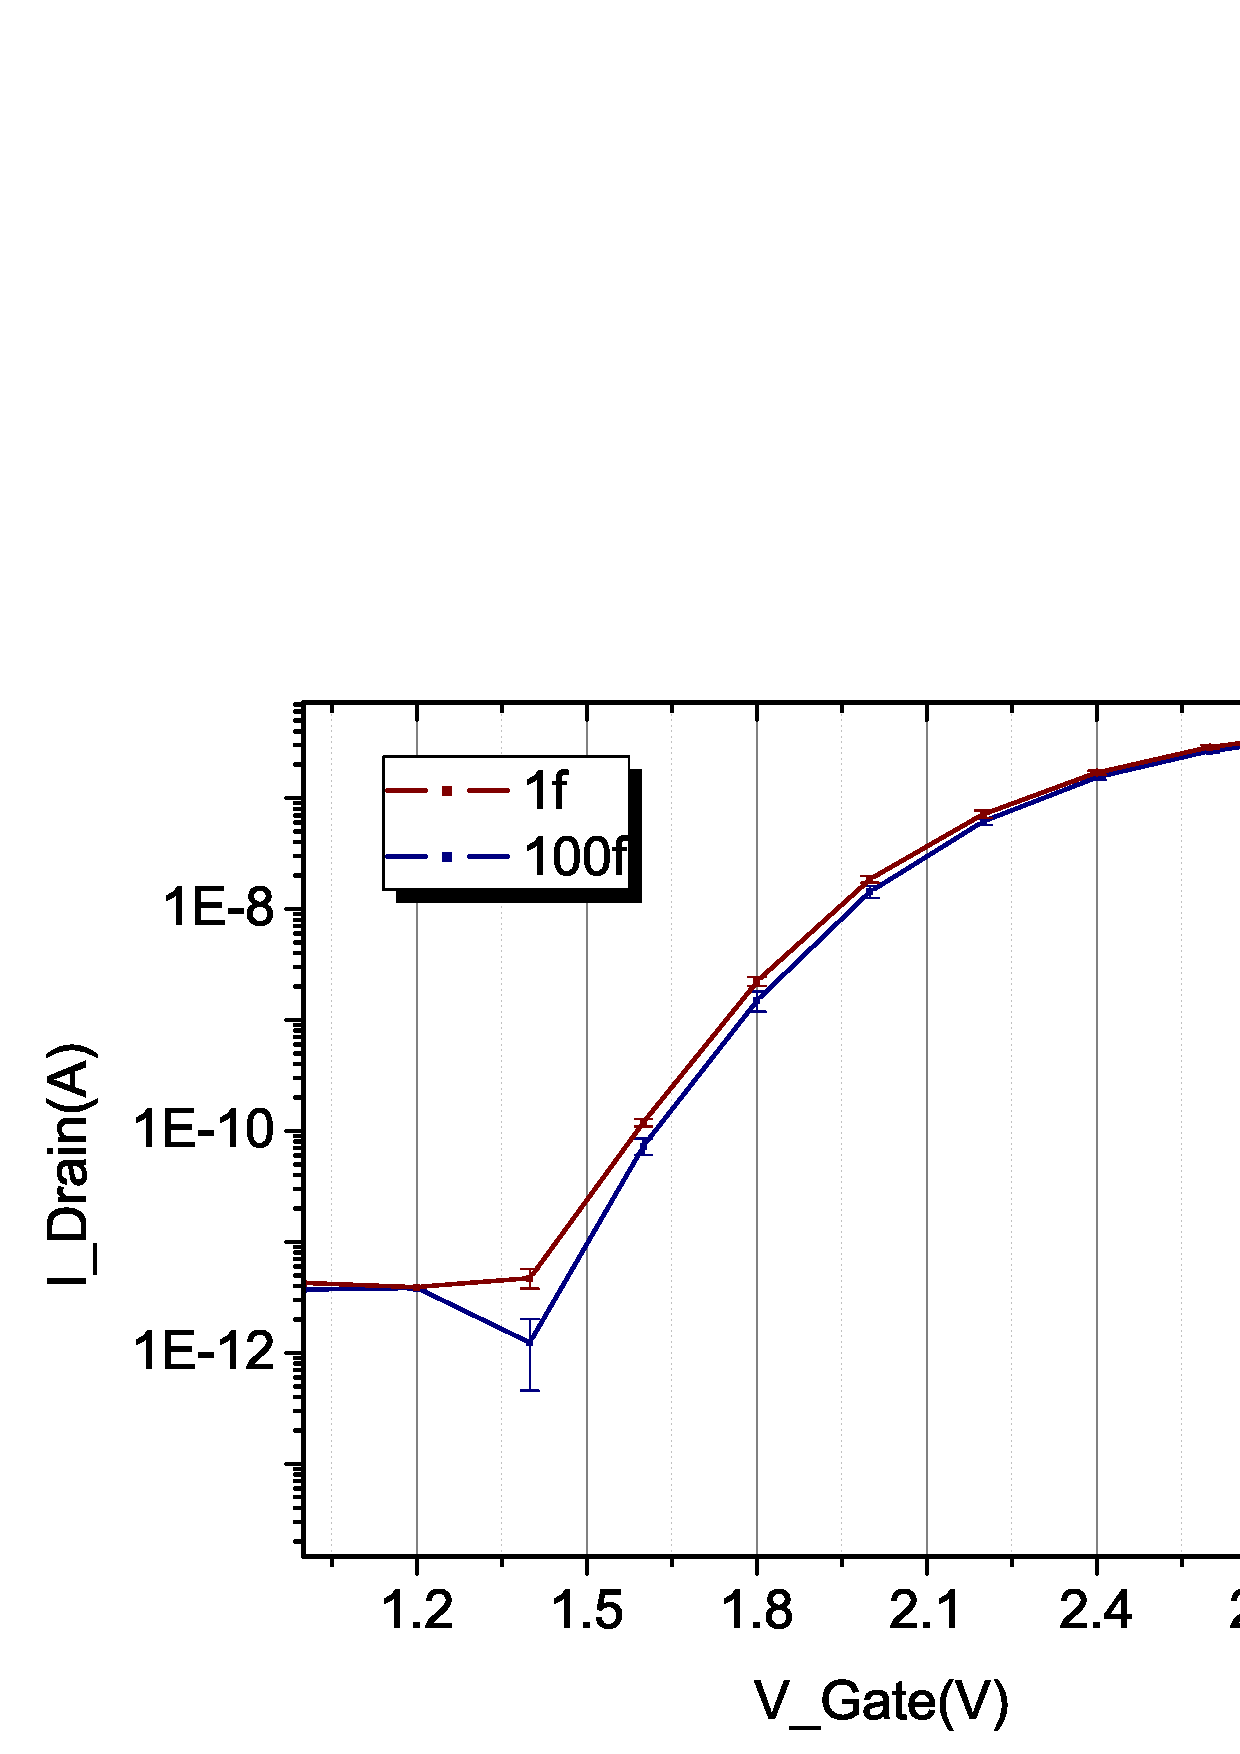
\includegraphics[width=1.8\textwidth]{images/chapter3/208_devices/L2-12_log.png}
            (e)
        \end{minipage}
        \hfill
        \begin{minipage}[t]{0.3\textwidth}
            \centering
            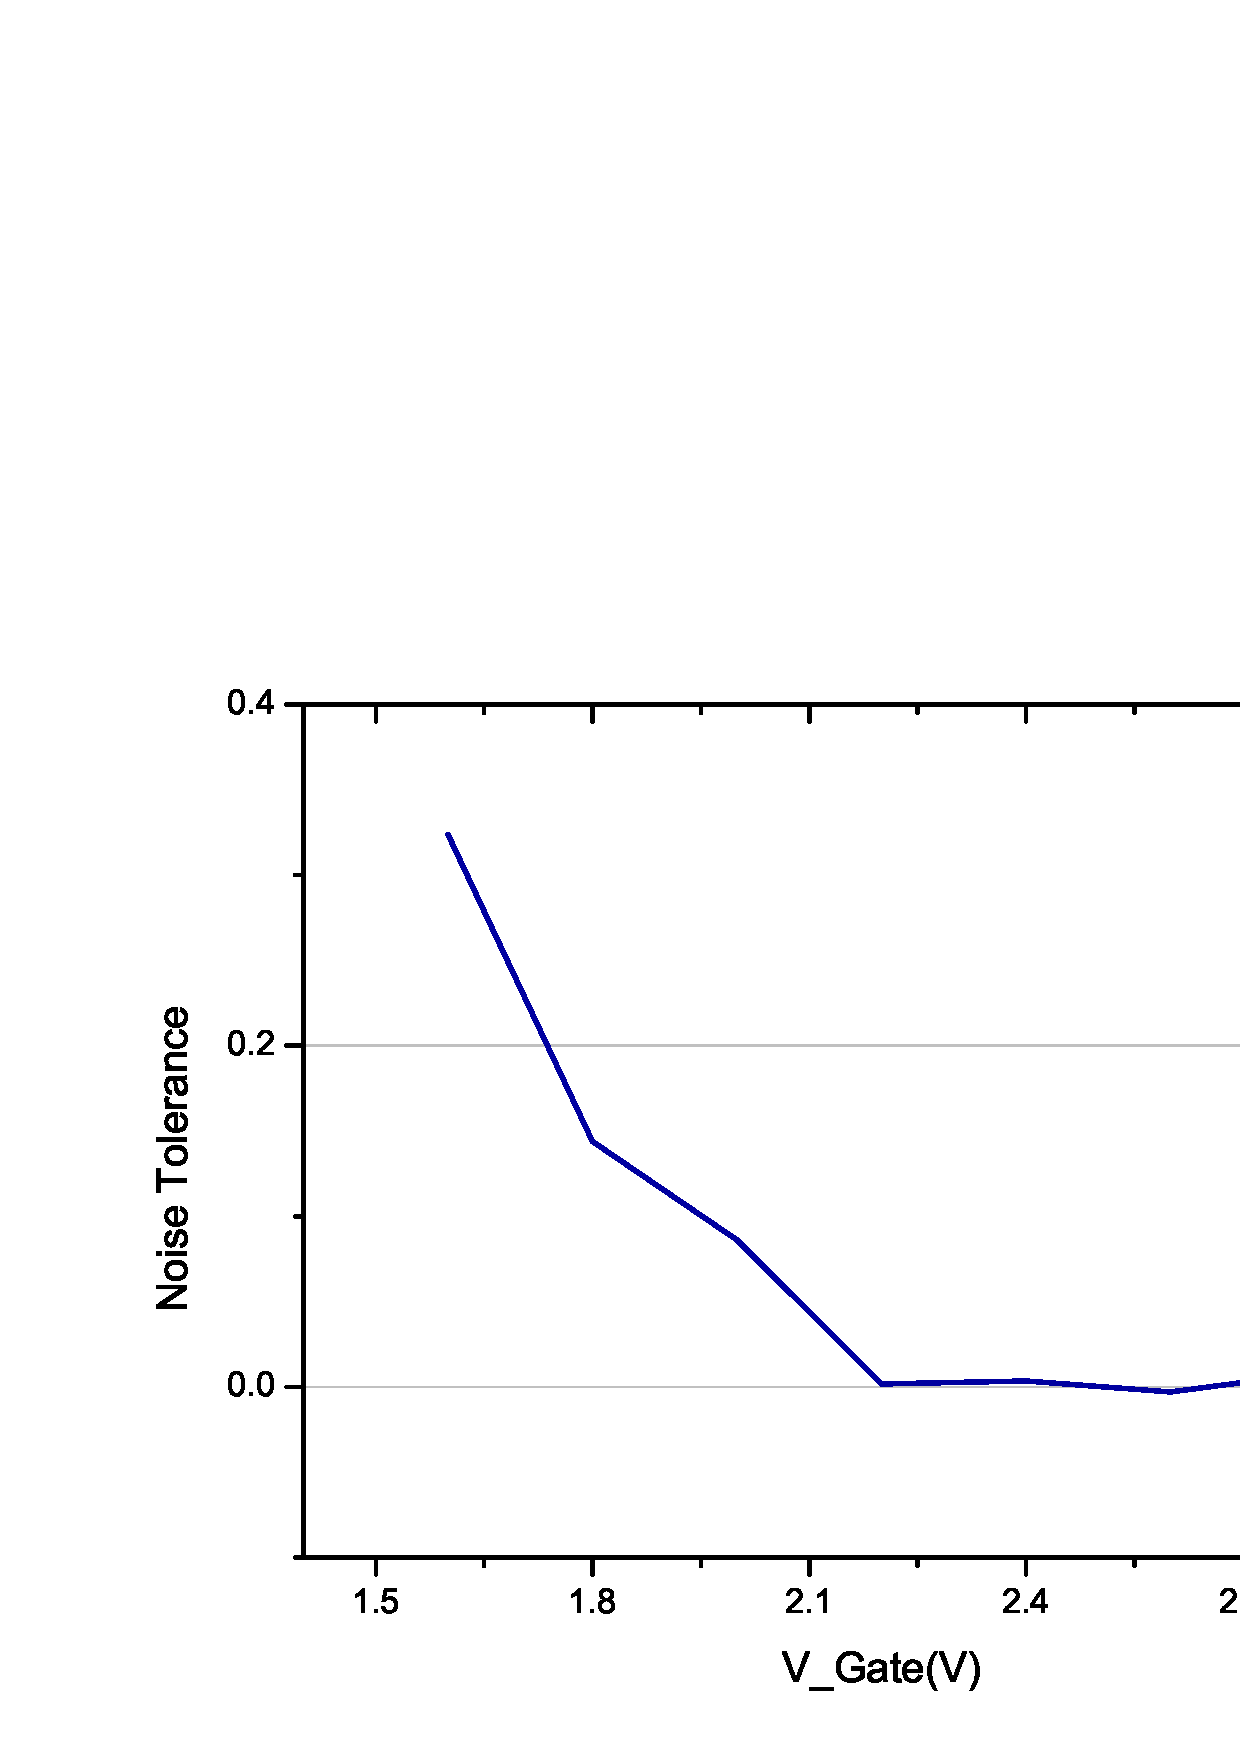
\includegraphics[width=1.6\textwidth]{images/chapter3/208_devices/L2-12_margin.png}
            (f)
        \end{minipage}

    \end{minipage}
    \caption{}
    \label{fig:SD_Device}
\end{figure}
\FloatBarrier

\subsection{$g_m$-$I_D$ Plot} \label{section:disparityBio}
We plot the $g_m$-$I_D$ curve with the data in Fig.\ref{fig:SD_allT}.
It clearly proves our two assumptions for dealing the disparity problem, which we have discussed in section.\ref{sec:assumpDiscuss}.

\begin{figure}[htb]
        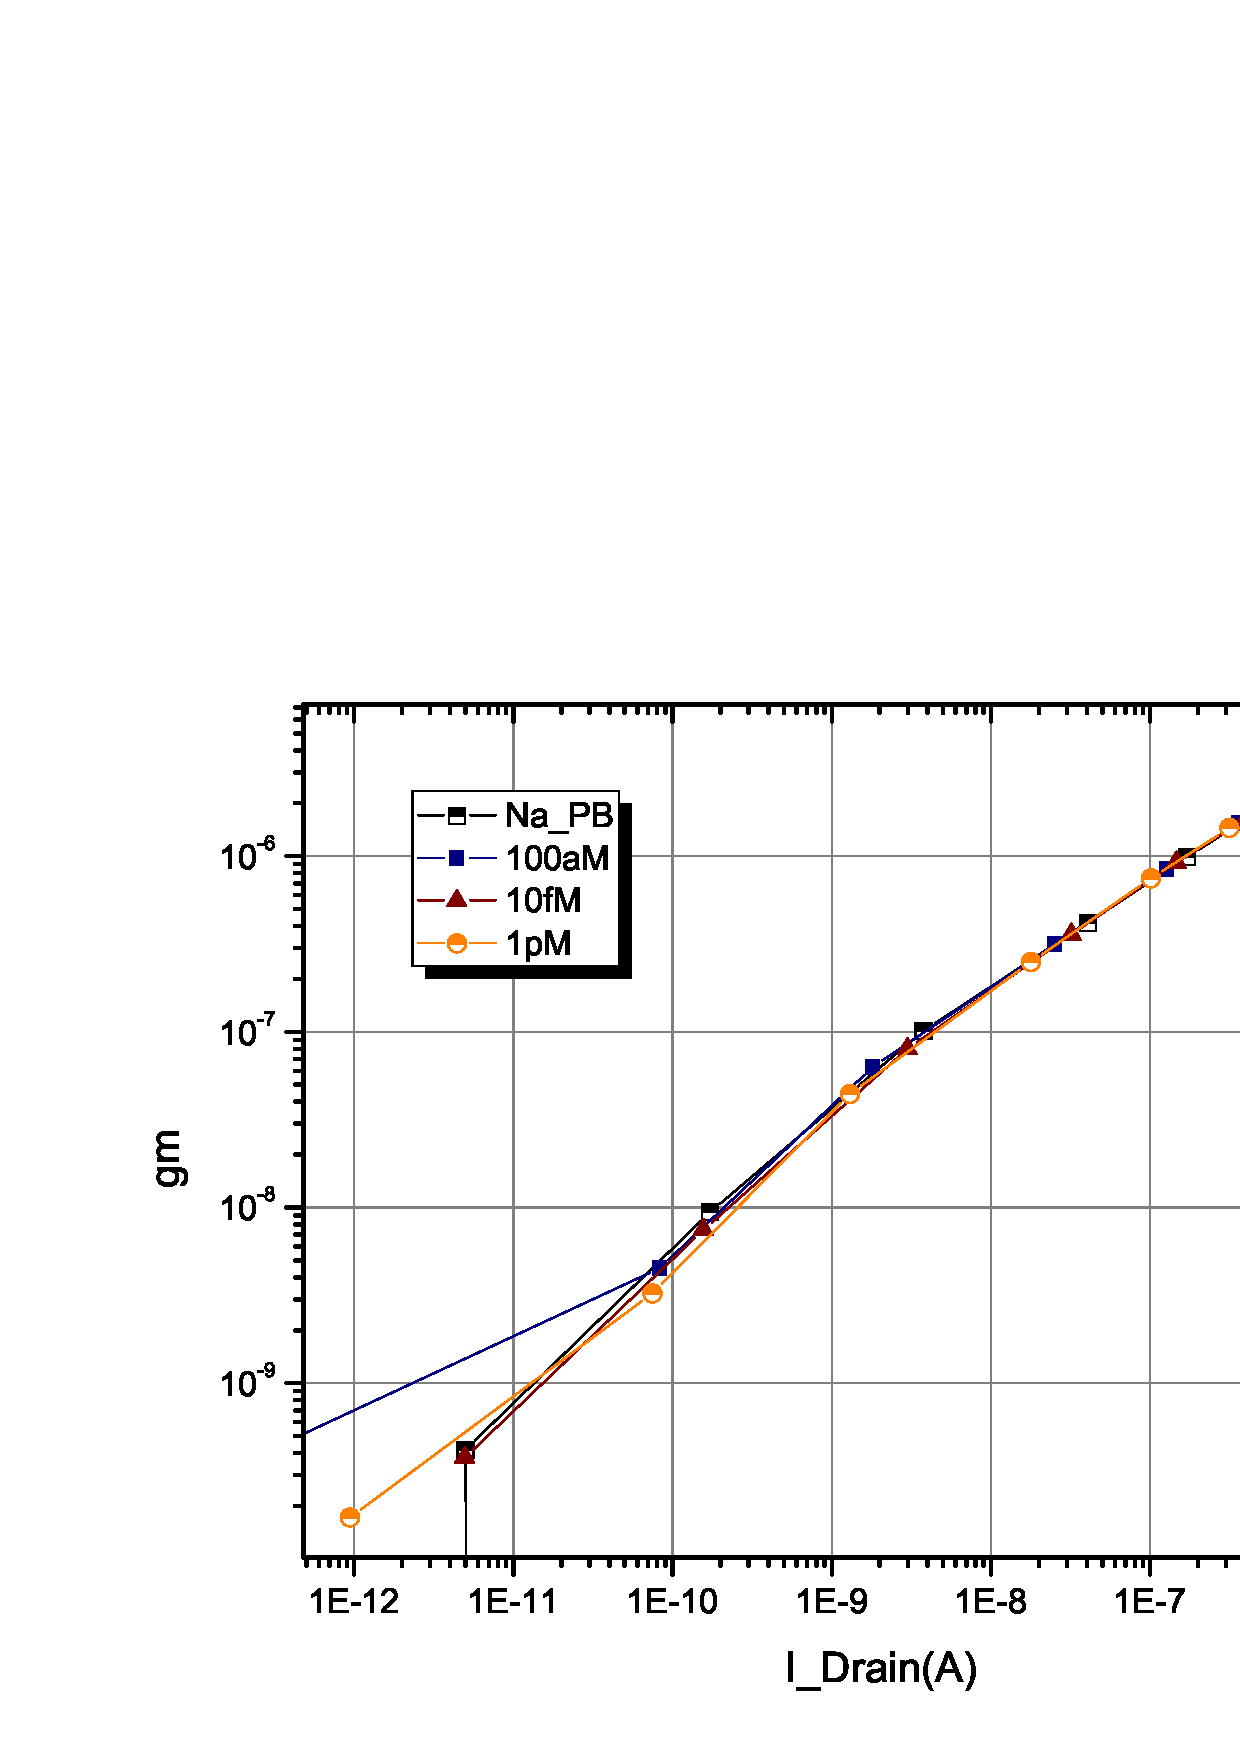
\includegraphics[width=1\textwidth]{images/chapter3/Id_Dev_bio.png}
    \caption{The $g_m$-$I_D$ curve obtained by the $I_D$-$V_G$ curve in Fig.\ref{fig:SD_allT}. The curves start splitting after $I_D$ > 1$\mu$A where the element may enter into strong inversion region.}
    \label{fig:gmId}
\end{figure}

In Fig.\ref{fig:gmId}, when $I_D$ is from 0.1nA to 1$\mu$A, we can observe that the $g_m$ of nanowire is almost independent of concentration and merely depends on $I_D$.
In fact, the curves start splitting after $I_D$ > 1$\mu$A.
It means the element is no longer in weak inversion region but enters into strong inversion region.

With the data from Fig.\ref{fig:gmId}, we may find the equivalent voltage value generated by the concentration difference based on the assumption 2 (section.\ref{sec:assumpDiscuss}).
\begin{table}[!htb]
    {\fontfamily{}\fontsize{10}{14}\selectfont
    \centering
    \begin{tabular}{l|c|c|c}
        Concentration Difference & Na\_PB - 100aM & 100aM - 10fM & 10fM - 1pM \\
        \hline
        Equivalent voltage value & $30mV - 40mV$ & $200mV - 280mV$ & $38mV - 60mV$ \\
    \end{tabular}
    \caption{The equivalent voltage value generated by the concentration difference. We obtained the data by the data from Fig.\ref{fig:gmId}. We divided the $I_D$ difference of different concentration by their $g_m$ ($\Delta I_D = g_m\Delta V_G$).}
    \label{tb:CdV}
    }
\end{table}
The values is changeable, which may result from the gate-coupling coefficient (Eq.\ref{eq:Ikappa}).










\section{Electrical Measurements}
This section presents the data analysis results.
The data are obtained from our measurements with the source meter (Keithley 2602).
To exclude the ion effect, we placed nanowire elements in dd-water instead of biomolecule solution.
And there is no DNA probe on the poly-Si channel surfaces.

\subsection{Front Gate and Back Gate}
Our nanowire has two gates available: floating gate (liquid gate) and back-gate.
We choose floating gate as the operation gate mainly because the floating gate can induce larger drain-current.
In other words, it has higher transconductance (Fig.\ref{fig:IdVgandgbsId}).
In our circuit design, nanowire is placed in a feedback loop where its transconductance is proportional to the loop gain (chapter 5).

\begin{figure}[!htbp]
    \centering
    \begin{minipage}[t][0.1\textheight]{0.4\textheight}
        \centering
        \def\svgwidth{12cm}
        \fontsize{6}{15}\selectfont
        \input {images/FgBg_Compare_Id.pdf_tex}
        (a)
    \end{minipage}
    \vfill
    \begin{minipage}[t][0.1\textheight]{0.4\textheight}
        \centering
        \def\svgwidth{12cm}
        \fontsize{6}{15}\selectfont
        \input {images/FgBg_Compare_Id_dev.pdf_tex}
        (b)
    \end{minipage}
    \caption{Comparison between the DC sweep of voltage on the floating gate and back gate. (a) $I_D$ (b) Transconductance ($g_m$): the derivative of $I_D$. The traansconductance of the floating gate is larger than the back gate.}
    \label{fig:IdVgandgbsId}
\end{figure}


There are some advantages of back-gate.
One of them is the ability to lower the 1/f noise \cite{C7, C8}.
But this only happens in a very high gate voltage, which is not practical in the integrated circuit design.

\subsection{Transconductance}
The most crucial parameter for our circuit design is the transconductance ($g_m$).
We acquire it by finding the partial derivative of $I_D$ of $V_{G}$.
Since in section.\ref{section:IdGm} we proved that $g_m$ is related to $I_D$, we plot the $g_m$-$I_D$ curve to reveal their relation (Fig.\ref{fig:pIdVg}(b)).

\begin{figure}[!htbp]
    \centering
    \begin{minipage}[t][0.1\textheight]{1\textwidth}
        \centering
        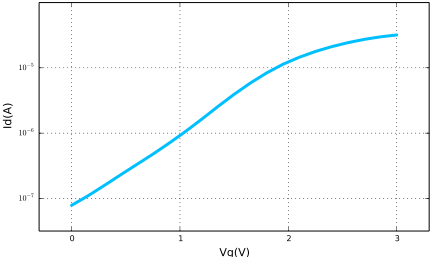
\includegraphics[width=0.6\textwidth,natwidth=610,natheight=442]{images/pIdVg.png}
        (a)
    \end{minipage}
    \hfill
    \begin{minipage}[t][0.1\textheight]{1\textwidth}
        \centering
        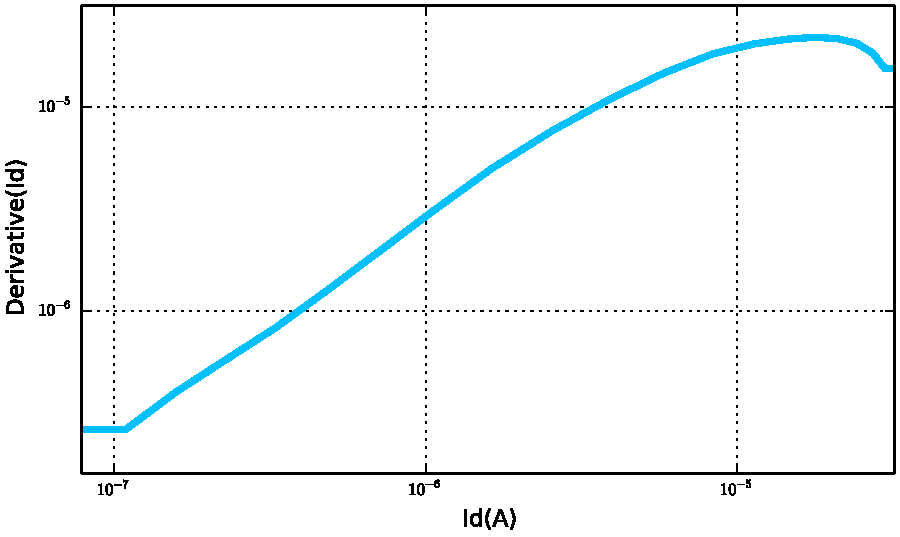
\includegraphics[width=0.6\textwidth,natwidth=610,natheight=442]{images/pIdgbs.png}
        (b)
    \end{minipage}
    \caption{Eelectrical response of a nanowire element. (a) Sweep $V_G$ and measure the $I_D$ changes. And by finding the transconductance ($g_m$): the derivative of $I_D$ of $V_G$, we plot (b) the $g_m$-$I_D$ curve}
    \label{fig:pIdVg}
\end{figure}

The $g_m$-$I_D$ plot indicates that there is a ``linear region'' where $g_m$ is proportional to $I_D$.
This corresponds to our induction (Eq.\ref{eq:gm_weak}).
We can recognize that our nanowire element is operated in weak inversion region when $I_D$ is less than 10$\mu$A.
Therefore, by the section.\ref{section:biasVg}, we decide our the $I_D$ of our nanowire should be operated below 10$\mu$A.

We also proved that the transconductance under this region is unaffected by the $V_{DS}$.

\begin{figure}[!htbp]
    \centering
    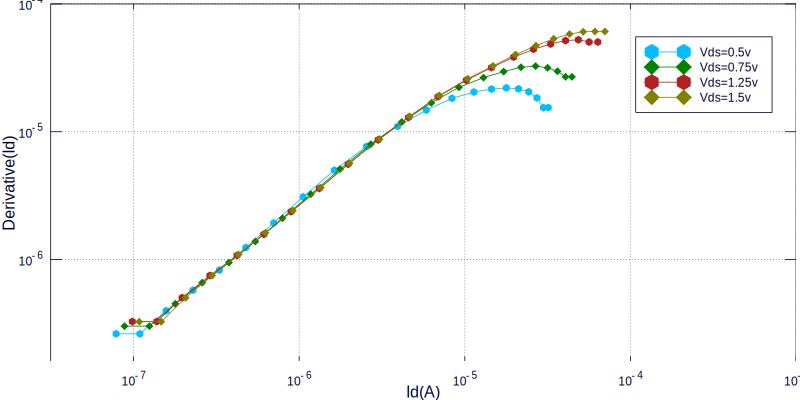
\includegraphics[width=0.8\textwidth]{images/pIdgbs_Vd.png}
    \caption{Id-transconductance with Vds variance}
    \label{fig:Idgbs_Vd}
\end{figure}

\subsection{Drain-to-source impedance ($r_{ds}$)}
In our circuit design, we keep $V_{DS}$ constant.
By the measurement in last section, 0.7 is enough to keep nanowire in saturation region for $V_G$ range from 0v to 3v.
However, due to the fabrication variance, the value varies from 0.75v to 1v.

We concern about how the $I_D$ effect $r_{ds}$.
The way we obtained $r_{ds}$ is as follows:
\begin{enumerate}
    \item Perform $I_D$-$V_G$ sweep with two different $V_D$.
    \item Find the difference of $I_D$ at each $V_G$ sweep point and divide it by the difference of $V_D$.
\end{enumerate}
The result is as Fig.\ref{fig:rds}

\begin{figure}[!htbp]
    \centering
    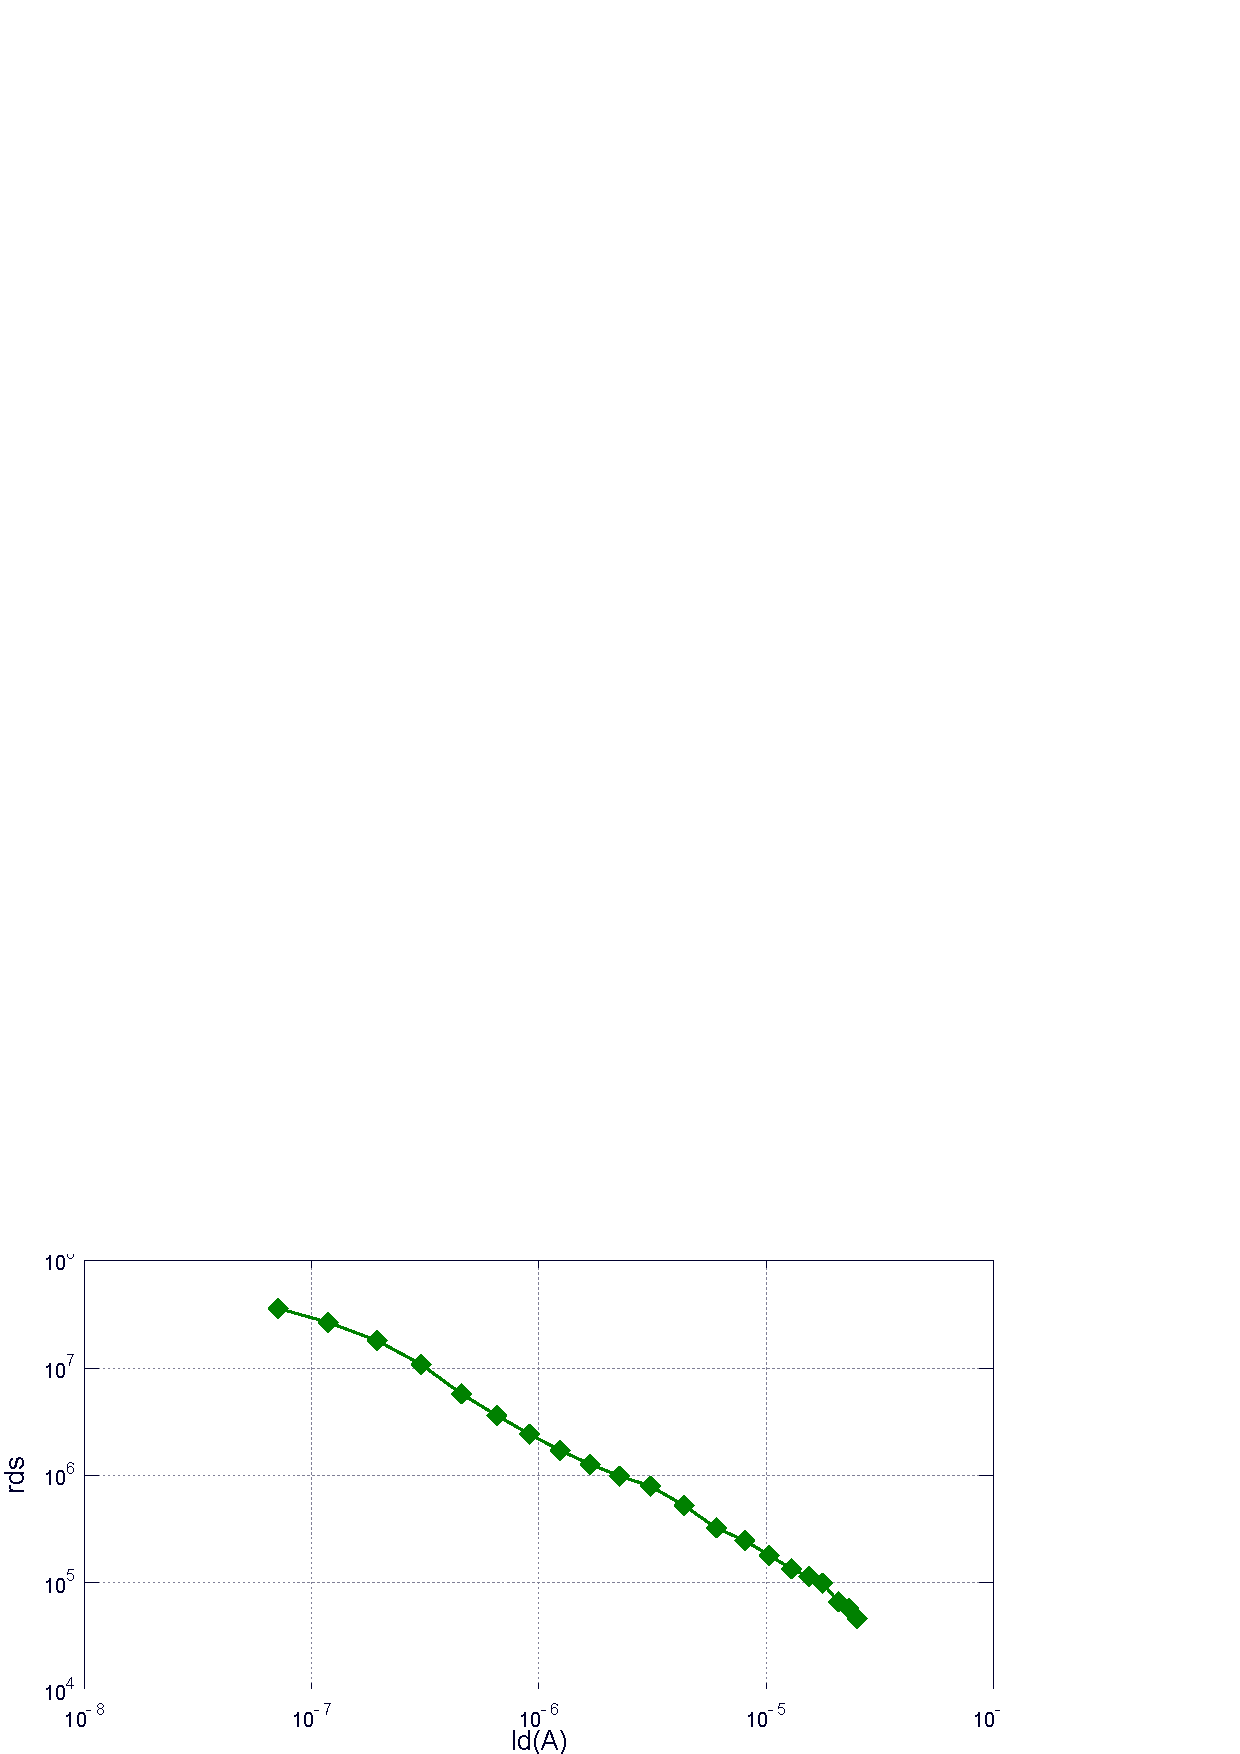
\includegraphics[width=0.8\textwidth]{images/chapter3/rds_I.png}
    \caption{$I_D$-$r_{ds}$ plot}
    \label{fig:rds}
\end{figure}


\section{Disparity Problem exists}
We measured two nanowire elements which lie on the same wafer and are immersed with the same testing PBS solution.
Below, the $g_m$-$I_D$ plot (Fig.\ref{fig:disparity}) shows that even the environment is same, two elements exhibit different electrical response.

\begin{figure}[!htbp]
    \centering
    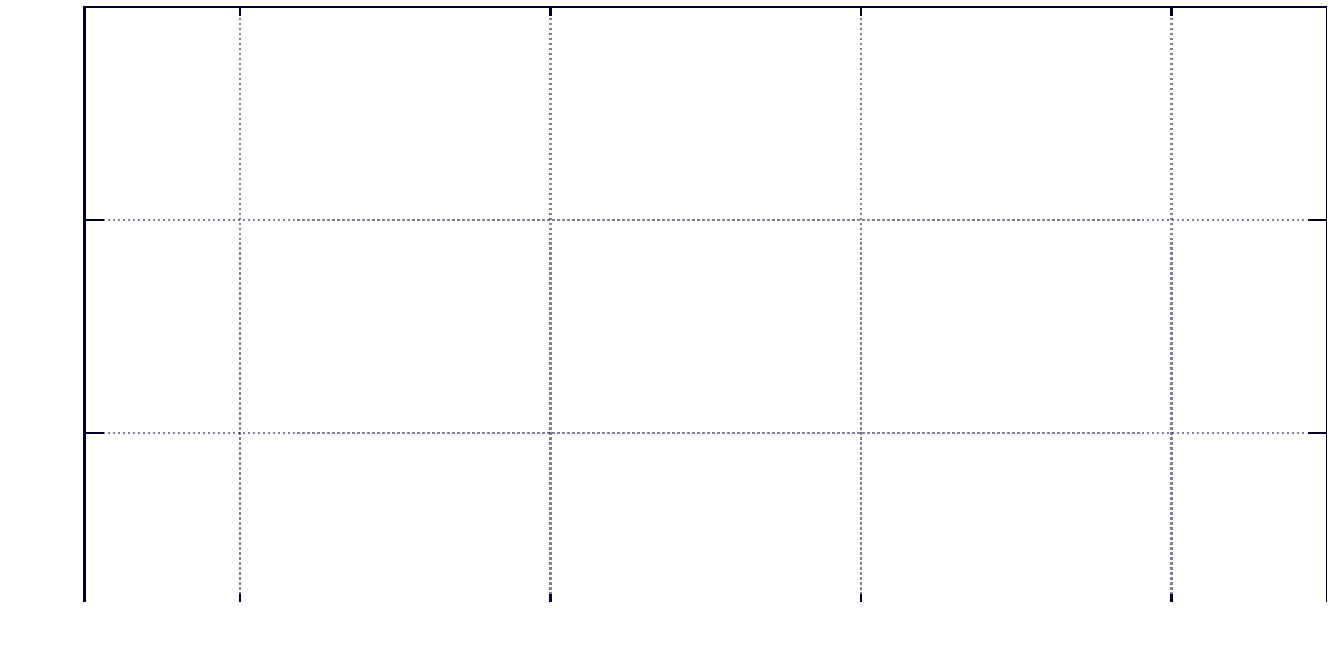
\includegraphics[width=0.67\textwidth] {images/pDisparity.png}
    \caption{Dusparity problem casue nanowire elements with same environment can exhibit different electrical responses.}
    \label{fig:disparity}
\end{figure}




\section{Conclusion and Design Spec}

Table.\ref{tb:NWcharacter} concludes the electrical characteristics of our nanowire.
\begin{table}[h!bp]
    {\fontfamily{}\fontsize{10}{14}\selectfont
    \centering
    \begin{tabular}{c|c|c|c|c}
        Operation Region & $I_D$ & $V_G$ & $g_m$ & $r_{ds}$ \\
        \hline
        Cut off & $< 100n A$ & $< 0 V$ & - & - \\
        weak inversion & $100n A$ - $10\mu A$ & $0 V$ - $2.5V$ & $200n $ - $20\mu$ & $50M\Omega$ - $200k\Omega$ \\
        strong inversion & $> 1\mu A$ & $> 2.2V$ & $20\mu$ - $30\mu$ & $< 200k\Omega $ \\
    \end{tabular}
    \caption{Element electrical characteristics. There are overlaps due to the element disparity}
    \label{tb:NWcharacter}
    }
\end{table}

We hence decide the detecting spec of the DC mode as in the table.\ref{tb:DCspec}.
\begin{table}[!htbp]
    {\fontfamily{}\fontsize{10}{14}\selectfont
    \centering
    \begin{tabular}{c|c}
        $I_D$ & $g_m$ \\
        \hline
        $100n A$ - $30\mu A$ & $200n $ - $20\mu$ \\
    \end{tabular}
    \caption{Detecting Spec of DC mode}
    \label{tb:DCspec}
    }
\end{table}

As for the AC mode, section.\ref{section:biasVg} suggests that the element should operated in the weak inversion region adjacent to the strong inversion region.
The table.\ref{tb:CdV} tells that the minimum equivalent input voltage ($\Delta V_G$) brought by concentration difference is $20mV$.
We integrate these informatino in table.\ref{tb:ACinput}.
\begin{table}[!htbp]
    {\fontfamily{}\fontsize{10}{14}\selectfont
    \centering
    \begin{tabular}{c|c|c}
        $I_D$ & $g_m$ & $\Delta V_G$ (min)\\
        \hline
        $600n A$ - $5\mu A$ & $1\mu $ - $10\mu$ & $20mV$\\
    \end{tabular}
    \caption{The summation of the nanowire characteristics when applied with AC mode circuit}
    \label{tb:ACinput}
    }
\end{table}
The Spec for AC mode circuit is as in table.\ref{tb:ACSpec}.
\begin{table}[!htbp]
    {\fontfamily{}\fontsize{10}{14}\selectfont
    \centering
    \begin{tabular}{c|c}
        Input referred Noise(V) & Amplification Rate (max) \\
        \hline
        $< 2m V$ & $10^7(\frac{V}{A})$\\
    \end{tabular}
    \caption{Spec of AC mode circuit}
    \label{tb:ACSpec}
    }
\end{table}





 

